% !TeX spellcheck = en_US
\documentclass[a4paper, 10pt, twoside, twocolumn]{scrartcl}
\special{papersize=210mm,297mm}
%%%%%%%%%%%%%%%%%%%%%%%%%%%%%%%%%%%%%%%%%%%%%%%%%%%%%%%%%%%%%%%%%%%%%%%%%%%%%%%
%% use the following parameter, when not using PDFLatex:                     %%
%%%%%%%%%%%%%%%%%%%%%%%%%%%%%%%%%%%%%%%%%%%%%%%%%%%%%%%%%%%%%%%%%%%%%%%%%%%%%%%
% %  dvips -t a4 ...                                                         %%
% %  ps2pdf -sPAPERSIZE=a4 ... # On Windows: ps2pdf -sPAPERSIZE#a4 ...       %%  
%%%%%%%%%%%%%%%%%%%%%%%%%%%%%%%%%%%%%%%%%%%%%%%%%%%%%%%%%%%%%%%%%%%%%%%%%%%%%%%

% uncomment or modify according to your operating system
% \usepackage[applemac]{inputenc} % european characters can be used (Mac OS)
%\usepackage[latin1]{inputenc} 
%\usepackage{fontspec}
%\usepackage{polyglossia}
\usepackage[utf8]{inputenc} % european characters can be used
\usepackage[T1]{fontenc} % hyphenation and accented letters
\usepackage{lmodern}
\usepackage{mathptmx} % times fonts
\usepackage[a4paper,twocolumn, twoside]{geometry}         
\usepackage{amsmath} % math environments, e.g. align, alignat, aligned
\usepackage{amsfonts} % additional fonts, e.g. \mathbb{}
\usepackage{amssymb} % additional math symbols
\usepackage{graphicx} % figure placement
\usepackage{tabularx}
\usepackage[usenames]{color} % color definitions
\usepackage{picture}
\usepackage{tikz} 
\usepackage{eso-pic}
\usepackage{fancyhdr} % header
\usepackage{calc}
\usepackage{hyperref}
\usepackage{ifthen}
\usepackage{forloop}
\usepackage{setspace}
\usepackage{xstring}
\usepackage[defaultsans]{opensans}
\usepackage{courier}
\newcounter{startpage}


\usepackage{booktabs}
\usepackage{subfig}

%%%%%%%%%%%%%%%%%%%%%%%%%%%%%%%%%%%%%%%%%%%%%%%%%%%%%%%%%%%%%%%%%%%%%%%%%%%%%%%%%%%%%%%%%%%%%%%%%%
%%
%% paper-specific data: to be filled out by paper-author!
%%
%%%%%%%%%%%%%%%%%%%%%%%%%%%%%%%%%%%%%%%%%%%%%%%%%%%%%%%%%%%%%%%%%%%%%%%%%%%%%%%%%%%%%%%%%%%%%%%%%%

\newcommand{\papertitle}{Modeling and Simulation of Electrical Ladder Systems with Julia}
\newcommand{\shortpapertitle}{Modeling and Simulation of Electrical Ladder Systems}
\newcommand{\mainauthors}{~Scholz~ {\itshape et al.~}} % for header  
\newcommand{\authors}{Stephan Scholz}

%\newcommand{\papertitle}{A New Template for Articles in\\ Simulation Notes Europe}
%\newcommand{\shortpapertitle}{A New Template for Articles in Simulation Notes Europe}
%\newcommand{\mainauthors}{~Preyser~ {\itshape et al.~}} % for header  
%\newcommand{\authors}{Johannes Tanzler\textsuperscript{1*}, Franz J. Preyser\textsuperscript{1}, Markus Wallerberger\textsuperscript{2}, Felix Breitenecker\textsuperscript{1}}
\newcommand{\institutes}{}


%% hyphenation exceptions:
%\hyphenation{ Julia }      

%%%%%%%%%%%%%%%%%%%%%%%%%%%%%%%%%%%%%%%%%%%%%%%%%%%%%%%%%%%%%%%%%%%%%%%%%%%%%%%%%%%%%%%%%%%%%%%%%%
%%%%%%%%%%%%%%%%%%%%%%%%%%%%%%%%%%%%%%%%%%%%%%%%%%%%%%%%%%%%%%%%%%%%%%%%%%%%%%%%%%%%%%%%%%%%%%%%%%

\include{./Macros/SNELatexTemplateMacrosVol23plus}

%%%%%%%%%%%%%%%%%%%%%%%%%%%%%%%%%%%%%%%%%%%%%%%%%%%%%%%%%%%%%%%%%%%%%%%%%%%%%%%%%%%%%%%%%%%%%%%%%%
%%%%%%%%%%%%%%%%%%%%%%%%%%%%%%%%%%%%%%%%%%%%%%%%%%%%%%%%%%%%%%%%%%%%%%%%%%%%%%%%%%%%%%%%%%%%%%%%%%


\begin{document}
\maketitle
\noindent
\parbox{\columnwidth}{
		\setlength{\fboxrule}{0.8pt}
		\setlength{\fboxsep}{1.7mm}
		{\color{SNE_GRAY}
\fbox{
	\parbox{0.92\columnwidth}{\setstretch{1.27}\rmfamily\footnotesize\fontsize{8.1pt}{1em}\selectfont
		~\\
		Here will be SNE-specific data positioned. \\
		To be filled out by editor. \\  
	}
		}}
		\setstretch{1.1}
		\vspace{-1.55 mm}
		\Abstract{%
%%%%%%%%%%%%%%%%%%%%%%%%%%%%%%%%%%%%%%%%%%%%%%%%%%%%%%%%%%%%%%%%%%%%%%%%%%%%%%%%%%%%%%%%%%%%%%%%%%
%% fill in abstract here:
... Electrical Circuit Ladders as ordinary differential equations ..
%%%%%%%%%%%%%%%%%%%%%%%%%%%%%%%%%%%%%%%%%%%%%%%%%%%%%%%%%%%%%%%%%%%%%%%%%%%%%%%%%%%%%%%%%%%%%%%%%%
		}
	}
	\normalsize
	\setstretch{1.1}
	\fontsize{10.3pt}{1.15em}\selectfont
	%%%%%%%%%%%%%%%%%%%%%%%%%%%%%%%%%%%%%%%%%%%%%%%%%%%%%%%%%%%%%%%%%%%%%%%%%%%%%%%%%%%%%%%%%%%%%%%%%%
	%% write paper - content as usual
	
\section*{Introduction}
\begin{itemize}
	\item Single circuits like RC and LC circuits are classic examples from school classes, e.g. physics to academic courses, e.g. control eng.. Not only for to describe the electrical behavior, but also emphasize connections to other scientific domains, e.g. waves.
	\item Single circuits in control eng. and system theory are used to exemplify the modeling via transfer functions. For simple circuits this approach is easy, but it becomes more difficult for larger circuits. They are used to introduce electronic filters, RC is low-pass; Bode plot.
	\item Electronic filter design; Cauer topology
	\item Matlab: \url{https://www.mathworks.com/help/rf/ref/lcladder.html}
	\item Telegrapher's equation
	\item Exists a lot of literature for frequency-based modeling
	\item In time domain standard approach is to build with Kirchhoff laws a differential-algebraic system of equations, see [tischendorf2001mathematical];
	\item Fractional order systems: Ewa PIOTROWSKA
	\item Port-Hamiltonian Systems, Dynamic Mode Decomposition [Daniel]
	\item Here: modeling via ordinary differential equations; second order differential equation
	\begin{equation}
		M \ddot{z}(t) + D \dot{z}(t) + S z(t) = G_{0} u(t) + G_{1} \dot{u}(t) + G_{2} \ddot{u}(t)
	\end{equation}
	\item Julia implementation; simulation	
	\item Focus here: main branch 2 series elements; shunt one element; in particular series of R \& L + shunt C
\end{itemize}	
	
\section{Circuit Modeling}

\begin{figure*}[t!]
	\centering
	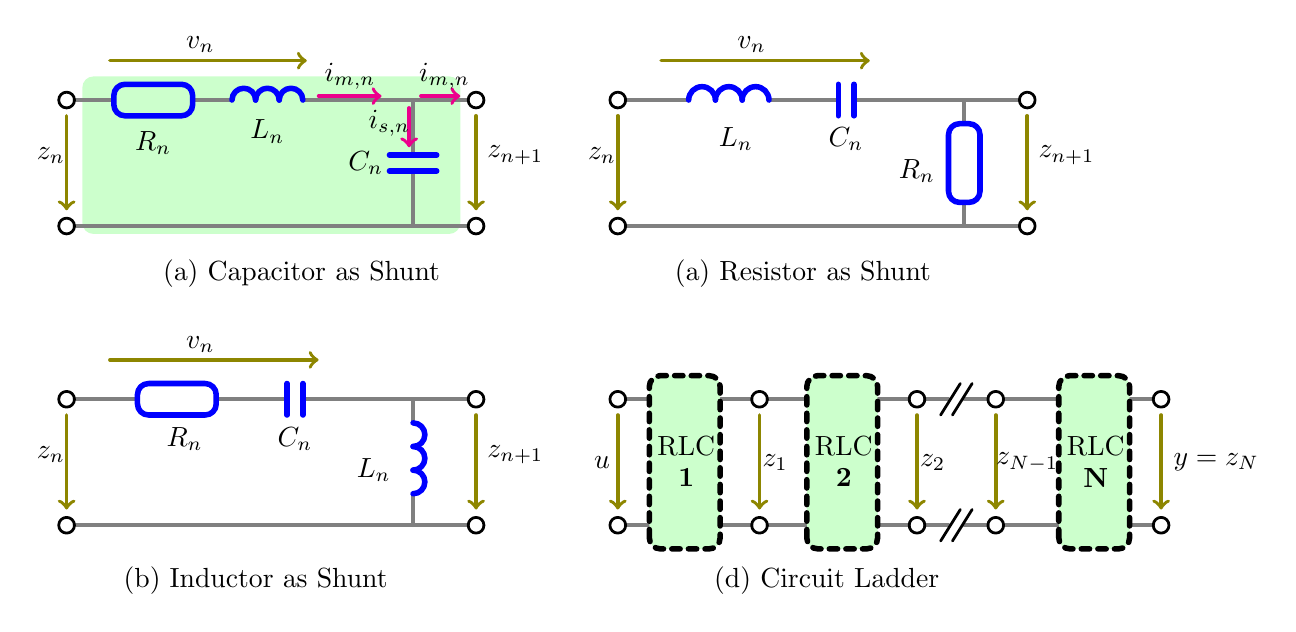
\begin{tikzpicture}[scale=1,line cap=round,line join=round,x=1.0cm,y=1.0cm]	
		\def\dxoff{7};
		\def\dyoff{3.8};
		
		\fill[color=green!20,opacity=10, rounded corners] (0.1,-1.7) rectangle (4.9,0.3);
		
		\draw[line width=1.3, color=gray] (0,0) -- (0.5,0);
		\draw[line width=1.3, color=gray] (1.5,0) -- (2.0,0);
		\draw[line width=1.3, color=gray] (2.9,0) -- (5.0,0);
		\draw[line width=1.3, color=gray] (4.3,0) -- (4.3,-0.7);
		\draw[line width=1.3, color=gray] (4.3,-0.9) -- (4.3,-1.6);
		\draw[line width=1.3, color=gray] (0,-1.6) -- (5.,-1.6);
		
		% Connector nodes
		\draw [line width=1.0] (-0.1, 0) circle [radius = 0.1];
		\draw [line width=1.0] ( 5.1, 0) circle [radius = 0.1];
		\draw [line width=1.0] (-0.1,-1.6) circle [radius = 0.1];
		\draw [line width=1.0] ( 5.1,-1.6) circle [radius = 0.1];
		
		% Resistor
		\draw[line width=2, color=blue,rounded corners] (0.5,-0.2) rectangle (1.5,0.2);
		
		
		% Inductor
		\draw[line width=2, color=blue] (2.0,0.) arc ( 180:0:0.15);
		\draw[line width=2, color=blue] (2.3,0.) arc ( 180:0:0.15);
		\draw[line width=2, color=blue] (2.6,0.) arc ( 180:0:0.15);
		
		% Capacitor
		\draw[line width=2, color=blue]  (4.0,-0.7) -- (4.6,-0.7);
		\draw[line width=2, color=blue]  (4.0,-0.9) -- (4.6,-0.9);
		
		\node at ( 1., -0.55) {$R_{n}$};
		\node at ( 2.45, -0.4) {$L_{n}$};
		\node at ( 3.7, -0.8) {$C_{n}$};
		
		
		% Currents
		\draw [->, line width=1.3, color=magenta] (3.1,0.05) -- (3.9,0.05);
		\draw [->, line width=1.3, color=magenta] (4.4,0.05) -- (4.9,0.05);
		\draw [->, line width=1.3, color=magenta] (4.25,-0.1) -- (4.25,-0.6);
		\node at (3.5, 0.3) {$i_{m,n}$};
		\node at (4.7, 0.3) {$i_{m,n}$};
		\node at (4.0, -0.3) {$i_{s,n}$};
		
		% Voltages
		\draw [->, line width=1.3, color=olive]	(-0.1, -0.2) -- (-0.1, -1.4);
		\draw [->, line width=1.3, color=olive]	( 5.1, -0.2) -- ( 5.1, -1.4);
		\draw [->, line width=1.3, color=olive]	( 0.45, 0.5) -- ( 2.95, 0.5);
		\node at (-0.3, -0.7) {$z_{n}$};
		\node at ( 5.6, -0.7)  {$z_{n+1}$};
		\node at ( 1.6, 0.7) {$v_{n}$};
		
		\node[right] at (1.0, -2.2) {(a) Capacitor as Shunt};
		
		
		
		%%% 2. Circuit: Resistor as Shunt %%%%%
		%%% 2. Circuit: Resistor as Shunt %%%%%
		%%% 2. Circuit: Resistor as Shunt %%%%%
		\draw[line width=1.3, color=gray] (\dxoff+0,0) -- (\dxoff+0.8,0);
		\draw[line width=1.3, color=gray] (\dxoff+1.82,0) -- (\dxoff+2.7,0);
		\draw[line width=1.3, color=gray] (\dxoff+2.9,0) -- (\dxoff+5.0,0);
		\draw[line width=1.3, color=gray] (\dxoff+4.3,0) -- (\dxoff+4.3,-0.3);
		\draw[line width=1.3, color=gray] (\dxoff+4.3,-1.3) -- (\dxoff+4.3,-1.6);
		\draw[line width=1.3, color=gray] (\dxoff+0,-1.6) -- (\dxoff+5.0,-1.6);
		
		
		% Nodes
		\draw [line width=1.0] (\dxoff-0.1, 0) circle [radius = 0.1];
		\draw [line width=1.0] (\dxoff+5.1, 0) circle [radius = 0.1];
		\draw [line width=1.0] (\dxoff-0.1,-1.6) circle [radius = 0.1];
		\draw [line width=1.0] (\dxoff+5.1,-1.6) circle [radius = 0.1];
		
		% Voltages
		\draw [->, line width=1.3, color=olive]	(\dxoff -0.1, -0.2) -- (\dxoff -0.1, -1.4);
		\draw [->, line width=1.3, color=olive]	(\dxoff +5.1, -0.2) -- (\dxoff +5.1, -1.4);
		\draw [->, line width=1.3, color=olive]	(\dxoff +0.45, 0.5) -- (\dxoff +3.1, 0.5);
		
		\node at (\dxoff -0.3, -0.7) {$z_{n}$};
		\node at (\dxoff+ 5.6, -0.7)  {$z_{n+1}$};
		\node at (\dxoff+ 1.6, 0.7) {$v_{n}$};
		
		% Inductor
		\draw[line width=2, color=blue] (\dxoff+0.8, 0) arc ( 180:0:0.17);
		\draw[line width=2, color=blue] (\dxoff+1.14, 0) arc ( 180:0:0.17);
		\draw[line width=2, color=blue] (\dxoff+1.48, 0) arc ( 180:0:0.17);
		
		% Capacitor
		\draw[line width=2, color=blue] (\dxoff+2.7,-0.2) -- (\dxoff+2.7,0.2);
		\draw[line width=2, color=blue] (\dxoff+2.9,-0.2) -- (\dxoff+2.9,0.2);
		
		% Resistor
		\draw[line width=2, color=blue,rounded corners] (\dxoff+4.1,-0.3) rectangle (\dxoff+4.5,-1.3);
		
		\node at (\dxoff+ 1.4, -0.5) {$L_{n}$};
		\node at (\dxoff+ 2.8, -0.5) {$C_{n}$};
		\node at (\dxoff+ 3.7, -0.9) {$R_{n}$};
		
		\node[right] at (\dxoff+0.5, -2.2) {(a) Resistor as Shunt};
		
		%%% 2. Circuit: Inductor as Shunt %%%%%
		%%% 2. Circuit: Inductor as Shunt %%%%%
		%%% 2. Circuit: Inductor as Shunt %%%%%
		
		\draw[line width=1.3, color=gray] (  0, 0-\dyoff) -- (0.8,0-\dyoff);
		\draw[line width=1.3, color=gray] (1.8, 0-\dyoff) -- (2.7,0-\dyoff);
		\draw[line width=1.3, color=gray] (2.9, 0-\dyoff) -- (5.0,0-\dyoff);
		\draw[line width=1.3, color=gray] (4.3, 0-\dyoff) -- (4.3,-0.3-\dyoff);
		\draw[line width=1.3, color=gray] (4.3,-1.2-\dyoff) -- (4.3,-1.6-\dyoff);
		
		\draw[line width=1.3, color=gray] (  0,-1.6-\dyoff) -- (5.0,-1.6-\dyoff);
		
		% Nodes
		\draw [line width=1.0] (-0.1, 0-\dyoff) circle [radius = 0.1];
		\draw [line width=1.0] ( 5.1, 0-\dyoff) circle [radius = 0.1];
		\draw [line width=1.0] (-0.1,-1.6-\dyoff) circle [radius = 0.1];
		\draw [line width=1.0] ( 5.1,-1.6-\dyoff) circle [radius = 0.1];
		
		% Voltages
		\draw [->, line width=1.3, color=olive]	(-0.1, -0.2-\dyoff) -- (-0.1, -1.4-\dyoff);
		\draw [->, line width=1.3, color=olive]	( 5.1, -0.2-\dyoff) -- ( 5.1, -1.4-\dyoff);
		\draw [->, line width=1.3, color=olive]	( 0.45, 0.5-\dyoff) -- ( 3.1, 0.5-\dyoff);
		
		\node at (-0.3, -0.7-\dyoff) {$z_{n}$};
		\node at ( 5.6, -0.7-\dyoff)  {$z_{n+1}$};
		\node at ( 1.6, 0.7-\dyoff) {$v_{n}$};
		
		% Resistor
		\draw[line width=2, color=blue,rounded corners] (0.8,-0.2-\dyoff) rectangle (1.8,0.2-\dyoff);
		
		% Capacitor
		\draw[line width=2, color=blue] (2.7,-0.2-\dyoff) -- (2.7,0.2-\dyoff);
		\draw[line width=2, color=blue] (2.9,-0.2-\dyoff) -- (2.9,0.2-\dyoff);
		
		% Inductor
		\draw[line width=2, color=blue] (4.3,-0.3-\dyoff) arc ( 90:-90:0.15);
		\draw[line width=2, color=blue] (4.3,-0.6-\dyoff) arc ( 90:-90:0.15);
		\draw[line width=2, color=blue] (4.3,-0.9-\dyoff) arc ( 90:-90:0.15);
		
		
		\node at ( 1.4, -0.5-\dyoff) {$R_{n}$};
		\node at ( 2.8, -0.5-\dyoff) {$C_{n}$};
		\node at ( 3.8, -0.9-\dyoff) {$L_{n}$};
		
		\node[right] at (0.5, -2.3-\dyoff) {(b) Inductor as Shunt};	
		
		
		%%%%% Cascaded RLC %%%%%%%%%%%%
		%%%%% Cascaded RLC %%%%%%%%%%%%
		%%%%% Cascaded RLC %%%%%%%%%%%%
		
		\draw[line width=1.3, color=gray] (\dxoff+0  , 0-\dyoff) -- (\dxoff+0.3, 0-\dyoff);
		\draw[line width=1.3, color=gray] (\dxoff+0  ,-1.6-\dyoff) -- (\dxoff+0.3,-1.6-\dyoff);
		\draw[line width=1.3, color=gray] (\dxoff+1.2, 0-\dyoff) -- (\dxoff+1.6, 0-\dyoff);
		\draw[line width=1.3, color=gray] (\dxoff+1.2,-1.6-\dyoff) -- (\dxoff+1.6,-1.6-\dyoff);
		\draw[line width=1.3, color=gray] (\dxoff+1.8, 0-\dyoff) -- (\dxoff+2.3, 0-\dyoff);
		\draw[line width=1.3, color=gray] (\dxoff+1.8,-1.6-\dyoff) -- (\dxoff+2.3,-1.6-\dyoff);
		\draw[line width=1.3, color=gray] (\dxoff+3.2, 0-\dyoff) -- (\dxoff+3.6, 0-\dyoff);
		\draw[line width=1.3, color=gray] (\dxoff+3.2,-1.6-\dyoff) -- (\dxoff+3.6,-1.6-\dyoff);			
		\draw[line width=1.3, color=gray] (\dxoff+3.8, 0-\dyoff) -- (\dxoff+4.1, 0-\dyoff);
		\draw[line width=1.3, color=gray] (\dxoff+3.8,-1.6-\dyoff) -- (\dxoff+4.1,-1.6-\dyoff);			
		\draw[line width=1.3, color=gray] (\dxoff+4.3, 0-\dyoff) -- (\dxoff+4.6, 0-\dyoff);
		\draw[line width=1.3, color=gray] (\dxoff+4.3,-1.6-\dyoff) -- (\dxoff+4.6,-1.6-\dyoff);
		\draw[line width=1.3, color=gray] (\dxoff+4.8, 0-\dyoff) -- (\dxoff+5.5, 0-\dyoff);
		\draw[line width=1.3, color=gray] (\dxoff+4.8,-1.6-\dyoff) -- (\dxoff+5.5,-1.6-\dyoff);
		\draw[line width=1.3, color=gray] (\dxoff+6.4, 0-\dyoff) -- (\dxoff+6.7, 0-\dyoff);
		\draw[line width=1.3, color=gray] (\dxoff+6.4,-1.6-\dyoff) -- (\dxoff+6.7,-1.6-\dyoff);	
		
		\draw [line width=1.0] (\dxoff+-0.1, 0-\dyoff) circle [radius = 0.1];
		\draw [line width=1.0] (\dxoff+-0.1,-1.6-\dyoff) circle [radius = 0.1];
		
		\draw [line width=1.0] (\dxoff+1.7, 0-\dyoff) circle [radius = 0.1];
		\draw [line width=1.0] (\dxoff+ 1.7,-1.6-\dyoff) circle [radius = 0.1];
		
		\draw [line width=1.0] (\dxoff+3.7, 0-\dyoff) circle [radius = 0.1];
		\draw [line width=1.0] (\dxoff+ 3.7,-1.6-\dyoff) circle [radius = 0.1];
		
		\draw [line width=1.0] (\dxoff+ 4.7, 0-\dyoff) circle [radius = 0.1];
		\draw [line width=1.0] (\dxoff+ 4.7,-1.6-\dyoff) circle [radius = 0.1];
		
		\draw [line width=1.0] (\dxoff+ 6.8, 0-\dyoff) circle [radius = 0.1];
		\draw [line width=1.0] (\dxoff+ 6.8,-1.6-\dyoff) circle [radius = 0.1];
		
		\draw [line width=1.0] (\dxoff+4,   -0.2-\dyoff) -- (\dxoff+4.25, 0.2-\dyoff);	
		\draw [line width=1.0] (\dxoff+4.15,-0.2-\dyoff) -- (\dxoff+4.4 , 0.2-\dyoff);	
		\draw [line width=1.0] (\dxoff+4,   -1.8-\dyoff) -- (\dxoff+4.25,-1.4-\dyoff);	
		\draw [line width=1.0] (\dxoff+4.15,-1.8-\dyoff) -- (\dxoff+4.4 ,-1.4-\dyoff);		
		
		\draw[dashed,line width=2,rounded corners, fill=green!20] (\dxoff+0.3,-1.9-\dyoff) rectangle (\dxoff+1.2,0.3-\dyoff);
		\draw[dashed,line width=2,rounded corners, fill=green!20] (\dxoff+2.3,-1.9-\dyoff) rectangle (\dxoff+3.2,0.3-\dyoff);
		\draw[dashed,line width=2,rounded corners, fill=green!20] (\dxoff+5.5,-1.9-\dyoff) rectangle (\dxoff+6.4,0.3-\dyoff);
		
		\node at (\dxoff+0.77,-0.6-\dyoff) {RLC};
		\node at (\dxoff+0.77,-1.0-\dyoff) {\textbf{1}};
		
		\node at (\dxoff+2.77,-0.6-\dyoff) {RLC};
		\node at (\dxoff+2.77,-1.0-\dyoff) {\textbf{2}};
		
		\node at (\dxoff+5.97,-0.6-\dyoff) {RLC};
		\node at (\dxoff+5.97,-1.0-\dyoff) {\textbf{N}};
		
		% Voltages
		\draw [->, line width=1.3, color=olive]	(\dxoff+-0.1, -0.2-\dyoff) -- (\dxoff+-0.1, -1.4-\dyoff);
		\draw [->, line width=1.3, color=olive]	(\dxoff+ 1.7, -0.2-\dyoff) -- (\dxoff+ 1.7, -1.4-\dyoff);
		\draw [->, line width=1.3, color=olive]	(\dxoff+ 3.7, -0.2-\dyoff) -- (\dxoff+ 3.7, -1.4-\dyoff);
		\draw [->, line width=1.3, color=olive]	(\dxoff+ 4.7, -0.2-\dyoff) -- (\dxoff+ 4.7, -1.4-\dyoff);
		\draw [->, line width=1.3, color=olive]	(\dxoff+ 6.8, -0.2-\dyoff) -- (\dxoff+ 6.8, -1.4-\dyoff);
		\node at (\dxoff+-0.3, -0.8-\dyoff) {$u$};
		\node at (\dxoff+ 1.9, -0.8-\dyoff) {$z_{1}$};
		\node at (\dxoff+ 3.9, -0.8-\dyoff) {$z_{2}$};
		\node at (\dxoff+ 5.1, -0.8-\dyoff) {$z_{N-1}$};
		\node at (\dxoff+ 7.5, -0.8-\dyoff)  {$y=z_{N}$};
		
		\node[right] at (\dxoff+1.0, -2.3-\dyoff) {(d) Circuit Ladder};
		
	\end{tikzpicture}
	\caption{Considered types of RLC circuits (a-c) and a Ladder of such circuits (d). The voltage at the last shunt is the output, $z_{n} = y$.}
	\label{fig:cascaded_rlc_circuits}
	
\end{figure*}

\begin{table}[b]
	\renewcommand{\arraystretch}{1.3}
	\centering
	\begin{tabularx}{\columnwidth}{l|l|l}\hlinewd{1.2pt}
		\textbf{Sym.} & \textbf{Explanation}        & \textbf{Domain} \\\hlinewd{1pt}
		$u$ & Input voltage & $[0,T] \rightarrow \mathbb{R}$ \\
		$y$ & Output voltage & $[0,T] \rightarrow \mathbb{R}$ \\
		$v_{n}$ & Voltage at main branch & $[0,T] \rightarrow \mathbb{R}$ \\
		$z_{n}$ & Voltage at shunt & $[0,T] \rightarrow \mathbb{R}$ \\
		$i_{m,n}$ & Current through main branch & $[0,T] \rightarrow \mathbb{R}$ \\
		$i_{s,n}$ & Current through shunt & $[0,T] \rightarrow \mathbb{R}$ \\
		$R_{n}$, $L_{n}$, $C_{n}$ & Resistor, Inductor, Capacitor & $\mathbb{R}_{>0} \setminus \{\infty\}$ \\ \hlinewd{1.2pt}
	\end{tabularx}
	\caption{Nomenclature of electrical states and quantities.}
	\label{table:el_symbols_explanation}
\end{table}

We begin the modeling with a single circuit of a ladder and demonstrate afterwards how to scale this approach for a specific RLC ladder. In our modeling approach, we consider nominal electronic components, i.e. a resistor has only a pure resistance without inductance or capacitance; and we assume a voltage source, which can supply an arbitrary signal. The voltages, currents and the quantities of the electrical components are noted in Table \ref{table:el_symbols_explanation}. The currents and voltages are functions of time, e.g. $u: [0,T] \rightarrow\mathbb{R}$ with final time $T>0$, while the quantities 	$R_{n}$, $L_{n}$ and $C_{n}$ are constant. We summarize the voltages at the shunt as 
\begin{equation}
	z = \left[z_{1}, z_{2}, \ldots, z_{N}\right]^{\top} \label{eq:z_voltages_shunt}
\end{equation}
and we consider the voltage at the last shunt as the output voltage $y(t) = z_{N}(t)$. We consider the currents and voltages to be sufficiently smooth, e.g. twice smoothly differentiable $i_{n}, v_{n}, z_{n} \in \mathcal{C}^{2}([0,T])$, and integrable, e.g. $\int_{0}^{T} i_{n}(\tau) d\tau < \infty$. According to Kirchhoff's voltage law, the $n$-th shunt voltage is identified by
\begin{equation}
	z_{n}(t) = v_{n+1}(t) + z_{n+1}(t) = \left[\sum_{k=n+1}^{N} v_{k}(t)\right] + z_{N} \label{eq:kirchhoff_voltage}
\end{equation}
and the input voltage in the first circuit is $z_{0} = u(t)$. As a ladder is a cascade of parallel circuits, the currents split up to the subsequent circuit $n+1$ and the shunt as
\begin{equation}
	i_{m,n}(t) =~ i_{m,n+1}(t) + i_{s,n}(t) ~=~ \sum_{k=n}^{N} i_{s,k}(t) \label{eq:kirchhoff_current}
\end{equation}
with the current in the final circuit $i_{m,N}(t) = i_{s,N}(t)$. We know that the ideal voltage $x:[0,\infty) \rightarrow \mathbb{R}$ across the electrical components is stated as 
\begin{align*}
	\text{Resistor:} \quad x(t) =&~ R ~ i(t) ~\text{,}\\
	\text{Inductor:} \quad x(t) =&~ L ~ \partial_{t} i(t) ~\text{,}\\
	\text{Capacitor:} \quad x(t) =&~ \frac{1}{C} ~ \int_{0}^{t} i(\tau) d\tau \text{.}
\end{align*}
These identities and compositions according to Eq. \eqref{eq:kirchhoff_voltage} are modeled as linear operator mappings 
\begin{equation*}
	\mathcal{F}\{i\}(t) = c_{0} ~ i(t) +  c_{1}~ \partial_{t} i(t) +  c_{2}~ \int_{0}^{t} i(\tau) d\tau 
\end{equation*}
where we distinguish these mappings for the main branch and shunt as
\begin{equation}
	v_{n}(t) = \mathcal{F}_{m,n} \left\{i_{m,n}\right\}(t) ~ \text{,} \quad 
	z_{n}(t) = \mathcal{F}_{s,n} \left\{i_{s,n}\right\}(t) \text{.} \label{eq:operator_maps}
\end{equation}
Subsequently, we apply the Kirchhoff laws and the operator mappings on the considered types of RLC ladders, see Fig. \ref{fig:cascaded_rlc_circuits}, in order to derive the systems of linear ordinary differential equations.



%In particular, we only consider linear mappings as 
%\begin{equation*}
%	\mathcal{F}\{c_{1} x_{1} + c_{2} x_{2}\} = c_{1} \mathcal{F}\{x_{1}\} + c_{2}\mathcal{F}\{x_{2}\} 
%\end{equation*}
%where mapping consists of differential and integral operators as
%\begin{equation*}
%%	\mathcal{F}\{x\}(t) = c_{0} x(t) +  c_{1}~ \partial_{t} x(t) +  c_{2}~ \partial_{t}^2 x(t) + c_{3} \int_{0}^{t} x(\tau) d\tau 
%\mathcal{F}\{x\}(t) = c_{0} x(t) +  c_{1}~ \partial_{t} x(t) +  c_{2}~ \int_{0}^{t} x(\tau) d\tau 
%\end{equation*}
%with $\partial_{t} := \frac{d}{dt}$ and $c_{0}, \ldots, c_{2}\in \mathbb{R}$ and arbitrary sufficiently smooth functions $x_{1}$, $x_{2}:[0,T]\rightarrow \mathbb{R}_{>0}$. 
%{\color{red} Konkreter fuer diesen Artikel; operator i zu z: RL-C; RC-L; LC-R}
%
%We evaluate the Kirchhoff laws (\ref{eq:kirchhoff_voltage}, \ref{eq:kirchhoff_current}) and the operator mappings \eqref{eq:operator_maps} in order to yield a relation between shunt voltages as
%\begin{align}
%	c_{2,n} ~ \partial_{t}^{2} z_{n-1}(t) + c_{1,n} ~ \partial_{t} z_{n-1}(t) + c_{0,n} ~ z_{n-1}(t) = \nonumber \\
%	 d_{0,n} ~ z_{n}(t) + d_{1,n} ~ \partial_{t} z_{n}(t) + d_{2,n} ~ \partial_{t}^{2} z_{n}(t) \text{.}
%\end{align}
%
%{\color{red} Until here it is general, now we assume a concrete RLC example}



\subsubsection*{RLC Ladder with Capacitor at Shunt}

In the first case, see Fig. \ref{fig:cascaded_rlc_circuits} (a), the voltage in the main branch with a resistor and an inductor is stated as
\begin{align}
	v_{n}(t) =&~ R_n i_{m,n}(t) + L_n \partial_{t} i_{m,n}(t) \nonumber \\ 
	=&~ (R_{n} + L_{n}\partial_{t}) ~ i_{m,n}(t) = \mathcal{F}_{m,n} \left\{i_{m,n}\right\}(t) \\ 
	=&~ \left[R_{n} + L_{n}\partial_{t}\right] ~ \sum_{k=n}^{N} i_{s,k}(t) \text{,} \label{eq:rlc_cap_volt_r_l}
\end{align}
and the shunt voltage is noted as
\begin{equation}
	z_{n}(t) =~ \frac{1}{C_{n}} \int_{0}^{t} i_{s,n}(\tau) d\tau ~~= \mathcal{F}_{s,n} \left\{i_{s,n}\right\}(t) \text{.} \label{eq:rlc_cap_volt_c}
\end{equation}
We compute the inverse operator mapping of Eq. \eqref{eq:rlc_cap_volt_c} as 
\begin{equation*}
	i_{s,n}(t) = \mathcal{F}_{s,n}^{-1} \left\{z_{n}\right\}(t) = C_{n} \partial_{t} z_{n}	
\end{equation*}
and insert it in Eq. \eqref{eq:rlc_cap_volt_r_l} to yield
\begin{align}
		v_{n}(t) =&~  \left[R_{n} + L_{n}\partial_{t}\right] ~ \sum_{k=n}^{N} C_{k} ~ \partial_{t} z_{k}(t) \nonumber \\
		=&~  \sum_{k=n}^{N} \left[ R_{n} ~  C_{k} ~  \partial_{t} + L_{n} ~  C_{k} ~ \partial^2_{t}\right] z_{k}(t) \label{eq:rlc_cap_volt_r_l_2}
\end{align}
We consider Kirchhoff's voltage law \eqref{eq:kirchhoff_voltage} with the voltage in main branch \eqref{eq:rlc_cap_volt_r_l_2} and so we calculate the shunt voltage for the $n$-th circuit, $n\in\{2,\ldots,N\}$ as the differential equation
\begin{align}
	0 =&~ \sum_{k=n}^{N} \left[ L_{n} C_{k} ~ \partial_{t}^2 z_{k}(t) + R_{n} C_{k} ~ \partial_{t} z_{k}(t)  \right] \nonumber \\
	&\qquad  + z_{n}(t) - z_{n-1}(t) \text{.} \label{eq:rl-c_shunt_ode_n}
\end{align}
For the first circuit of the ladder, we have $u(t) = z_{0}(t)$ and so we note
\begin{equation}
	u(t) =~ \sum_{k=1}^{N} \left[ L_{1} C_{k} ~ \partial_{t}^2 z_{k}(t) + R_{1} C_{k} ~ \partial_{t} z_{k}(t)  \right] + z_{1}(t) \text{.} \label{eq:rl-c_shunt_ode_0}
\end{equation}


%We present two more circuit types: firstly a resistor as shunt and secondly an inductor as shunt, see Fig. \ref{fig:rlc_resistor_inductor}. 

\subsubsection*{Resistor as Shunt}
In the second case, see Fig. \ref{fig:cascaded_rlc_circuits} (b), we have an inductor and a capacitor in the main branch and a resistor as shunt. Hence, we note the voltages as 
\begin{align} % Type LC-R
	v_{n}(t) =&~ L_n ~ \partial_{t} i_{m,n}(t) + \frac{1}{C_{n}} \int_{0}^{t} i_{m,n}(\tau) d\tau \nonumber \\
	=&~ \mathcal{F}_{m,n} \left\{i_{m,n}\right\}(t) \qquad\text{and} \label{eq:lc-r_volt_main} \\
	z_{n}(t) =&~ R_n ~ i_{s,n}(t)  = \mathcal{F}_{s,n} \left\{i_{s,n}\right\}(t) \text{.} \label{eq:lc-r_volt_shunt}
\end{align}
We differentiate both sides of Eq. \eqref{eq:lc-r_volt_main} and we apply Eq. (\ref{eq:kirchhoff_current}, \eqref{eq:lc-r_volt_shunt}) to obtain
\begin{align*}
	\partial_{t} v_{n}(t) =&~ \left[L_n \partial_{t}^2 + \frac{1}{C_{n}}\right] i_{m,n}(t) \\
	=&~ \left[L_n \partial_{t}^2 + \frac{1}{C_{n}}\right] \left[  \sum_{k=n}^{N} i_{s,k}(t)  \right] \\
	=&~ \left[L_n \partial_{t}^2 + \frac{1}{C_{n}}\right] \left[  \sum_{k=n}^{N} \frac{z_{k}(t)}{R_{k}} \right] \text{.}
\end{align*}
We evaluate the Kirchhoff voltage law \eqref{eq:kirchhoff_voltage} and we  note the differential equation of the $n$-th circuit 
for  $k\in\{2,\ldots,N\}$ as 
\begin{align}
	0 =&~ \sum_{k=n}^{N} \left[ \frac{L_{n}}{R_{k}} ~ \partial_{t}^2 z_{k}(t) + \frac{z_{k}(t)}{R_{k}~C_{n}} \right] \\
	&\qquad   + \partial_{t} \left[z_{n}(t) - z_{n-1}(t)\right] \label{eq:lc-r_shunt_ode_n}
\end{align}
for $n\in\{2,\ldots,N\}$, and for $n=1$ we have
\begin{equation}
	\partial_{t} u(t) =~ \sum_{k=1}^{N} \left[ \frac{L_{1}}{R_{k}} ~ \partial_{t}^2 z_{k}(t) + \frac{z_{k}(t)}{R_{k}~C_{1}} \right] + \partial_{t} z_{1}(t) \text{.} \label{eq:lc-r_shunt_ode_0}
\end{equation}

\subsubsection*{Inductor as Shunt}
In case of the third circuit type, see Fig. \ref{fig:cascaded_rlc_circuits} (c), we note the voltages as 
\begin{align}
	v_{n}(t) =&~ R_n ~ i_{m,n}(t) + \frac{1}{C_{n}} \int_{0}^{t} i_{m,n}(\tau) d\tau \text{,} \label{eq:rc-l_volt_main}  \\ 
	z_{n}(t) =&~ L_n ~ \partial_{t} i_{s,n}(t) \text{.} \label{eq:rc-l_volt_shunt}
\end{align}
We differentiate Eq. \eqref{eq:rc-l_volt_main} two times and we insert $\partial_{t} i_{s,n}(t)$ from Eq. \eqref{eq:rc-l_volt_shunt}. Hence, we yield the identity
\begin{align*}
	\partial_{t}^2 v_{n}(t) =&~ \left[R_n ~ \partial_{t} + \frac{1}{C_{n}} \right] \partial_{t}  i_{m,n}(t) \\
	=&~ \left[R_n ~ \partial_{t} + \frac{1}{C_{n}} \right]  \left[ \sum_{k=n}^{N} \frac{z_{k}(t)}{L_{k}}  \right] \text{.}
\end{align*}
In a analog way as before, we note the differential equation of the $n-th$ circuit as
\begin{equation}
	0 =~  \partial_{t}^2 \left[z_{n}(t) - z_{n-1}(t)\right] + \sum_{k=n}^{N} \left[ \frac{\partial_{t} z_{k}(t)}{R_{n} ~ L_{k}} + \frac{z_{k}(t)}{L_{k}~C_{n}} \right] \label{eq:rc-l_shunt_ode_n}
\end{equation}
and for the first circuit, we note
\begin{equation}
	\partial_{t}^2 u(t) =~  \partial_{t}^2 z_{1}(t) + \sum_{k=n}^{N} \left[ \frac{\partial_{t} z_{k}(t)}{R_{1} ~ L_{k}} + \frac{z_{k}(t)}{L_{k}~C_{1}} \right] \text{.} \label{eq:rc-l_shunt_ode_0}
\end{equation}







\section{System of Differential Equations}

\begin{itemize}
	\item Instead of $R$ and $L$ maybe $\ell$ $r$
	\item First-order systems: naming of $A_{1}$ and $A_{2}$ >> $P=[p_{n,k}]$ and $Q=[q_{n,k}]$??
\end{itemize}

\subsection{Second-Order System}

We collect the equations of the shunt voltages, e.g. Eq.  (\ref{eq:rl-c_shunt_ode_0}, \ref{eq:rl-c_shunt_ode_n}), and we arrange them as a system of second order equations
\begin{equation}
	M~ \ddot{z}(t) + D~ \dot{z}(t) + S~ z(t) = G ~ \mu(t)
	\label{eq:rlc_second_order_1}
\end{equation}
with matrices $M = \left[ m_{n,k} \right]$, $D = \left[ d_{n,k} \right]$ and  $S = \left[ s_{n,k} \right]$, and vectors $z$ as in Eq. \eqref{eq:z_voltages_shunt} and  $G = [1, 0, \ldots, 0]^{\top}$. The indices of our matrix elements denote a row $n\in \{1,\ldots,N\}$ and column $k\in \{1,\ldots,N\}$. This index notation refers to the indices in the voltage differential equations, e.g. Eq. (\ref{eq:rl-c_shunt_ode_n}, \ref{eq:rl-c_shunt_ode_0}) etc. The input signal $\mu(t)$ identifies either $u(t)$ for circuit \ref{fig:cascaded_rlc_circuits} (a), $\partial_{t} u(t) = \dot{u}(t)$  for circuit (b) or  $\partial_{t}^2 u(t) = \ddot{u}(t)$ for circuit (c).

The symbols of these matrices, $M$, $D$ and $S$, refer to the mass, damping and stiffness in mechanical systems. Our modeling approach of the second-order systems results in two types of matrices: upper triangular shapes and lower finite difference stencils, see the matrix shapes in Fig. \ref{fig:matrix_shapes}. The upper triangular matrices have a shape like
\begin{equation}
	\tilde{T} = 
	\begin{pmatrix}
		a_{1} b_{1} & a_{1} b_{2} & \cdots &  a_{1} b_{N-1} & a_{1} b_{N} \\
		0 			& a_{2} b_{2} & \cdots &  a_{2} b_{N-1} & a_{2} b_{N} \\
		\vdots			& \ddots	  & \ddots &  \vdots        & 	\vdots	  \\
		&			  &        & a_{N-1} b_{N-1}& a_{N-1} b_{N} \\
		0			&	\cdots		  &        &	0            & a_{N} b_{N} 
	\end{pmatrix}
	\label{eq:triangular_matrix} 
\end{equation}
where our coefficients $(a_{n}, b_{n})$ stand for the related electrical coefficients, $R_{n}$, $L_{n}$, $C_{n}$ and their reciprocals; and the finite difference stencil is
\begin{equation*}
	\tilde{F} = 
	\begin{pmatrix}
		1 & 0 & \cdots &  &  0\\
		-1 			& 1 & 0 &   & \vdots  \\
		0 & \ddots	  & \ddots & \ddots  & 	 \\
		\vdots &			  &     -1  & 1 &  0 \\
		0 &	\cdots		  &     0   & -1  & 1 
	\end{pmatrix} 
	\label{eq:finite_diff_stencil} 
\end{equation*}
The matrix entries for each circuit type are noted in Table \ref{table:overview_matrix_entries}. The triangular matrix structure corresponds to a spatially discrete integration and the finite difference shape to a differentiation.  We assume, $R_{n}$, $L_{n}$, $C_{n} \in \mathbb{R}_{>0} \setminus \{\infty\}$ and so the resulting triangular matrices are invertible. Hence, we are able to reformulate the second-order system via inverse matrix multiplication as first-order system. 


\begin{figure}[t!]
	\centering
	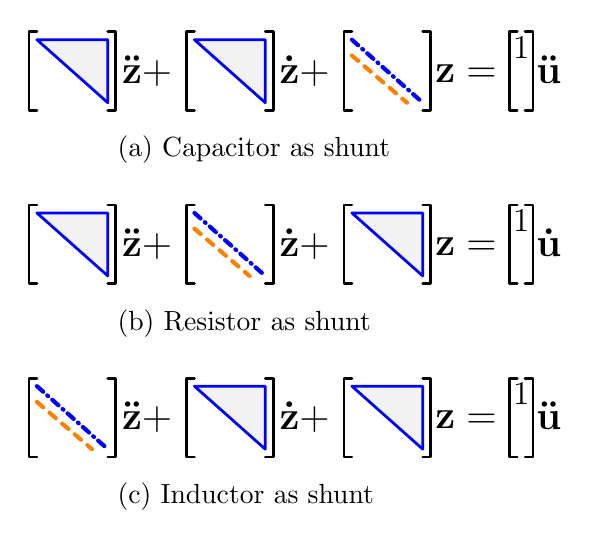
\begin{tikzpicture}[scale=1,line cap=round,line join=round,x=1.0cm,y=1.0cm]	
		\def\dx{2};
		\def\dy{2.2};
		
		\foreach \i in {0, 1, 2}
		{
			\draw[line width=1.0] (0.1+\i*\dx,0+\dy) -- (0+\i*\dx,0+\dy) -- (0+\i*\dx,1+\dy) -- (0.1+\i*\dx,1+\dy);
			\draw[line width=1.0] (1.0+\i*\dx,0+\dy) -- (1.1+\i*\dx,0+\dy) -- (1.1+\i*\dx,1+\dy) -- (1.0+\i*\dx,1+\dy);
		}
		\node at (1.5,0.5+\dy) {\Large $\mathbf{\ddot{z}}+$};
		\node at (1.5+\dx,0.5+\dy) {\Large $\mathbf{\dot{z}}+$};
		\node at (1.55+2*\dx,0.47+\dy) {\Large $\mathbf{z}=$};
		
		\draw[line width=1, color=blue, fill=gray!10] (0.1, 0.9+\dy) -- (1.0, 0.9+\dy) -- (1.0, 0.1+\dy) -- cycle;
		\draw[line width=1, color=blue, fill=gray!10] (0.1+\dx, 0.9+\dy) -- (1.0+\dx, 0.9+\dy) -- (1.0+\dx, 0.1+\dy) -- cycle;
		\draw[dash dot,line width=1.5, color=blue] (0.1+2*\dx,0.9+\dy) -- (1.+2*\dx,0.1+\dy);
		\draw[dashed,line width=1.5, color=orange] (0.1+2*\dx,0.7+\dy) -- (0.8+2*\dx,0.1+\dy);
		\draw[line width=1.0] (0.2+3*\dx,0+\dy) -- (0.1+3*\dx,0+\dy) -- (0.1+3*\dx,1+\dy) -- (0.2+3*\dx,1+\dy);
		\draw[line width=1.0] (0.3+3*\dx,0+\dy) -- (0.4+3*\dx,0+\dy) -- (0.4+3*\dx,1+\dy) -- (0.3+3*\dx,1+\dy);
		\node at (0.25+3*\dx,0.8+\dy) {\large $1$};
		\node at (0.6+3*\dx,0.52+\dy) {\Large $\mathbf{\ddot{u}}$};
		
		\node[right] at (1.0, -0.5+\dy) {(a) Capacitor as shunt};
		
		
		\foreach \i in {0, 1, 2}
		{
			\draw[line width=1.0] (0.1+\i*\dx,0) -- (0+\i*\dx,0) -- (0+\i*\dx,1) -- (0.1+\i*\dx,1);
			\draw[line width=1.0] (1.0+\i*\dx,0) -- (1.1+\i*\dx,0) -- (1.1+\i*\dx,1) -- (1.0+\i*\dx,1);
		}
		\node at (1.5,0.5) {\Large $\mathbf{\ddot{z}}+$};
		\node at (1.5+\dx,0.5) {\Large $\mathbf{\dot{z}}+$};
		\node at (1.55+2*\dx,0.47) {\Large $\mathbf{z}=$};
		\draw[line width=1, color=blue, fill=gray!10] (0.1, 0.9) -- (1.0, 0.9) -- (1.0, 0.1) -- cycle;
		\draw[line width=1, color=blue, fill=gray!10] (0.1+2*\dx, 0.9) -- (1.0+2*\dx, 0.9) -- (1.+2*\dx, 0.1) -- cycle;
		\draw[dash dot,line width=1.5, color=blue] (0.1+\dx,0.9) -- (1.+\dx,0.1);
		\draw[dashed,line width=1.5, color=orange] (0.1+\dx,0.7) -- (0.8+\dx,0.1);
		\draw[line width=1.0] (0.2+3*\dx,0) -- (0.1+3*\dx,0) -- (0.1+3*\dx,1) -- (0.2+3*\dx,1);
		\draw[line width=1.0] (0.3+3*\dx,0) -- (0.4+3*\dx,0) -- (0.4+3*\dx,1) -- (0.3+3*\dx,1);
		\node at (0.25+3*\dx,0.8) {\large $1$};
		\node at (0.6+3*\dx,0.52) {\Large $\mathbf{\dot{u}}$};
		
		\node[right] at (1.0, -0.5) {(b) Resistor as shunt};
		
		
		\def\dy{-2.2};
		\foreach \i in {0, 1, 2}
		{
			\draw[line width=1.0] (0.1+\i*\dx,0+\dy) -- (0+\i*\dx,0+\dy) -- (0+\i*\dx,1+\dy) -- (0.1+\i*\dx,1+\dy);
			\draw[line width=1.0] (1.0+\i*\dx,0+\dy) -- (1.1+\i*\dx,0+\dy) -- (1.1+\i*\dx,1+\dy) -- (1.0+\i*\dx,1+\dy);
		}
		\node at (1.5,0.5+\dy) {\Large $\mathbf{\ddot{z}}+$};
		\node at (1.5+\dx,0.5+\dy) {\Large $\mathbf{\dot{z}}+$};
		\node at (1.55+2*\dx,0.47+\dy) {\Large $\mathbf{z}=$};
		\draw[dash dot,line width=1.5, color=blue] (0.1,0.9+\dy) -- (1.,0.1+\dy);
		\draw[dashed,line width=1.5, color=orange] (0.1,0.7+\dy) -- (0.8,0.1+\dy);
		\draw[line width=1, color=blue, fill=gray!10] (0.1+\dx, 0.9+\dy) -- (1.0+\dx, 0.9+\dy) -- (1.0+\dx, 0.1+\dy) -- cycle;
		\draw[line width=1, color=blue, fill=gray!10] (0.1+2*\dx, 0.9+\dy) -- (1.0+2*\dx, 0.9+\dy) -- (1.+2*\dx, 0.1+\dy) -- cycle;
		\draw[line width=1.0] (0.2+3*\dx,0+\dy) -- (0.1+3*\dx,0+\dy) -- (0.1+3*\dx,1+\dy) -- (0.2+3*\dx,1+\dy);
		\draw[line width=1.0] (0.3+3*\dx,0+\dy) -- (0.4+3*\dx,0+\dy) -- (0.4+3*\dx,1+\dy) -- (0.3+3*\dx,1+\dy);
		\node at (0.25+3*\dx,0.8+\dy) {\large $1$};
		\node at (0.6+3*\dx,0.52+\dy) {\Large $\mathbf{\ddot{u}}$};
		
		\node[right] at (1.0, -0.5+\dy) {(c) Inductor as shunt};
		
	\end{tikzpicture}
	\caption{Matrix shapes of alternative RLC circuit ladders.}
	\label{fig:matrix_shapes}
\end{figure}


\begin{table}[b]
	\renewcommand{\arraystretch}{1.3}
	\centering
	\caption{\MakeUppercase{Matrix Entries of Second-Order ODE}}
	\begin{tabular}{l | c c c}
		\toprule
		Shunt & $m_{n,k}$ & $d_{n,k}$ & $s_{n,k}$ \\
		\midrule
		Capacitor &
		$L_{n}~C_{k} ~~\text{if} ~ n \leq k$ 
		& $	R_{n}~C_{k} ~~\text{if} ~ n \leq k$ & 
		$\begin{matrix}
			1 ~\text{if} ~ n = k ~\text{,}\\
			-1 ~\text{if} ~ n = k+1
		\end{matrix}$ \\
		Resistor &
		$\frac{L_{n}}{R_{k}} ~~\text{if} ~ n \leq k$ &
		$\begin{matrix}
			1 ~\text{if} ~ n = k ~\text{,}\\
			-1 ~\text{if} ~ n = k+1
		\end{matrix}$ & 
		$\frac{1}{R_{k}~ C_{n}}~~\text{if} ~ n \leq k$ \\
		Inductor &
		$\begin{matrix}
			1 ~\text{if} ~ n = k ~\text{,}\\
			-1 ~\text{if} ~ n = k+1
		\end{matrix}$ &
		&
		\\
		\bottomrule
	\end{tabular}
	\label{table:overview_matrix_entries}
\end{table}

\subsection{First-Order System}
Subsequently, we reformulate Eq. \eqref{eq:rlc_second_order_1} to yield a first-order system in the common state space formulation. Hence, we firstly find
\begin{equation}
	\ddot{z}(t) + M^{-1}~D ~ \dot{z}(t) + M^{-1}~S ~ z(t) = M^{-1}~G ~ \mu(t)	 \label{eq:rlc_second_order_2}
\end{equation}
where we specify the matrices 
\begin{equation}
P = -M^{-1}~S \quad \text{and} \quad Q := -M^{-1}~D	\label{eq:first_order_submatrices_P_Q}
\end{equation}
and vector $\tilde{G}:= M^{-1}~G$, and we note secondly 
\begin{equation*}
	\ddot{z}(t) = P ~ z(t)  + Q ~ \dot{z}(t) + \tilde{G} ~ z(t) \text{.}
\end{equation*}
We introduce the new states $x_{1}(t) = z(t)$, $x_{2}(t) = \partial_{t} z(t)$ and we formulate the state space as 
\begin{align}
	\begin{pmatrix}
	\dot{x}_{1} \\	
	\dot{x}_{2}
	\end{pmatrix}
	=
	\begin{pmatrix}
		0 & I \\
		P & Q
	\end{pmatrix}
	\begin{pmatrix}
		{x}_{1} \\	
		{x}_{2}
	\end{pmatrix}
	+
	\begin{pmatrix}
		0  \\
		\tilde{G}
	\end{pmatrix}
	u(t)\text{.}
\end{align}
If matrix $M$ in Eq. (\ref{eq:rlc_second_order_1},\ref{eq:rlc_second_order_2}) is not well conditioned, i.e. $M$ has a large condition number $\kappa = \frac{\max_{i} |\lambda_{i}|}{\min_{i} |\lambda_{i}|} \gg 1$ with eigenvalues $\lambda_{i}$ and $i \in [1,\ldots,2N]$, then a numerical computation of sub-matrices $P$ and $Q$ might be prone to numerical errors; and hence we need to have a closed form of these sub-matrices. In Fig. \ref{fig:matrix_multiplication}, we sketch the matrix multiplications from Eq. \eqref{eq:first_order_submatrices_P_Q} for the discussed matrix shapes in Eq. (\ref{eq:triangular_matrix}, \ref{eq:finite_diff_stencil}); and subsequently, we discuss these computations in detail. 

\subsection*{Inverse Triangular Matrix and Finite Difference Stencil}
To compute sub-matrices $P$ and $Q$ for circuit types (a) and (b), we need to find the inverse of their triangular matrix $M$. It has the shape as noted in Eq. \eqref{eq:triangular_matrix} and its inverse is found as the upper finite difference stencil shape 
\begin{align*}
	\tilde{T}^{-1} = 
	\begin{pmatrix}
		\frac{1}{a_{1} ~ b_{1}} & \frac{-1}{a_{2} ~ b_{1}} & 0  						& \cdots & 0 \\[1ex]
		0 						 &   \frac{1}{a_{2} ~ b_{2}} & \frac{-1}{a_{3} ~ b_{2}} &  & \vdots \\
		\vdots 				 		 &  \ddots 					 & \ddots 					 & \ddots & 0	 \\
		&  & 0 & \frac{1}{a_{N-1} ~ b_{N-1}} & \frac{-1}{a_{N} ~ b_{N-1}} \\[1ex]
		0  & \cdots 	& &  			0			   & \frac{1}{a_{N} ~ b_{N}} 
	\end{pmatrix} \text{.}
\end{align*}
A multiplication of $\tilde{T}^{-1}$ with a lower finite difference stencil, see Fig. \ref{fig:matrix_multiplication} (a), results in a tridiagonal shaped matrix as in Eq. \eqref{eq:finite_diff_stencil} with a $n$-th row vector elements 
\begin{equation*}
	\left[ \frac{-1}{a_{n}~ b_{n}},  \underbrace{\frac{1}{a_{n}~ b_{n}} + \frac{1}{a_{n+1}~ b_{n}}}_{n = k ~~ \text{(row = col.)}}, \frac{-1}{a_{n+1}~ b_{n}}\right] \text{.}
\end{equation*}
In case of circuit type (a), we compute sub-matrix $P$ with this matrix multiplication, while for circuit type (b), we find sub-matrix $Q$ with such a tridiagonal shape.
%{\color{red} with an upper triangular matrix, like matrix $S$ for circuit (a) or $D$ for circuit (b), results in an upper triangular matrix again; where a multiplication with the finite difference stencil, $S$ for circuit (a) or $D$ for circuit (b), results in a tridiagonal shaped matrix. }

\subsection*{Inverse Triangular and Triangular Matrix}
We consider the inverse triangular matrix $\tilde{T}^{-1}$ as above and we specify the second upper triangular matrix as $U = \left[\alpha_{n}~b_{k}\right]$ analog to $T$ in  Eq. \eqref{eq:triangular_matrix}, with equal $b_{k}$ but different $a_{n} \neq \alpha_{n}$. We evaluate the multiplication elementwise as 
\begin{align}
	\left. \tilde{T}^{-1} \cdot U \right\lvert_{n,k} = 
	\begin{cases}
		\frac{\alpha_{n}}{a_{n}} \quad &\text{if} ~ n = k ~\text{,}\\[1ex]
		\left[\frac{\alpha_{n}}{a_{n}} - \frac{\alpha_{n+1}}{a_{n+1}} \right] \frac{b_{k}}{b_{n}}\quad &\text{if} ~ n < k ~\text{,}\\[1ex]
		0 \quad &\text{else}
	\end{cases}
\end{align}
and so we have in general a triangular matrix. However, if we have a scaling $\alpha_{n} = \epsilon a_{n}$ for all $n \in \{1,\ldots,N\}$ with $\epsilon \in \mathbb{R}$, then we yield a pure diagonal matrix
\begin{equation*}
	\tilde{T}^{-1} \cdot U = \epsilon~I \text{.}
\end{equation*}
We emphasize that this matrix multiplication is relevant for circuit type (a) to yield sub-matrix $Q$; and for circuit type (b) to compute $P$.

\subsection*{Inverse Finite Difference Stencil and Triangular Matrix}
The third matrix multiplication is only applied for the first-order systems of circuit type (c). Here, we invert the finite difference stencil $\tilde{F}$ and we obtain a lower triangular matrix
\begin{equation*}
	\tilde{F}^{-1} =
	 	\begin{pmatrix}
	 	1 & 0  &  0\\
	 	\vdots 	& \ddots &  0 \\
	 	1 &	\cdots	 &     1 
	 \end{pmatrix} \text{.}
\end{equation*}
We multiply this lower triangular matrix with $\tilde{T}$ as in Eq. \eqref{eq:triangular_matrix} and we evaluate the results elementwise as
\begin{equation}
	\left. \tilde{F}^{-1} \cdot \tilde{T}  \right\rvert_{n,k} = b_{k} \sum_{i=1}^{\min\{n,k\}} a_{i} \text{.}
\end{equation}
If all values of $b_{n}$ are equal, then this matrix multiplication results in a shape
\begin{equation*}
	\tilde{F}^{-1} \cdot \tilde{T} =
	\begin{pmatrix}
		 & \text{---} & v_{1} & \text{---} & \\
		| & & \text{---} & v_{2} & \text{---} \\
		v_{1} & | & & &  \\
		| & v_{2} & & \ddots & \\
		& | &  & & \\
	\end{pmatrix}
\end{equation*}
where the values of the $n$-th row and column coincide.

\begin{figure}[t!]
	\centering
	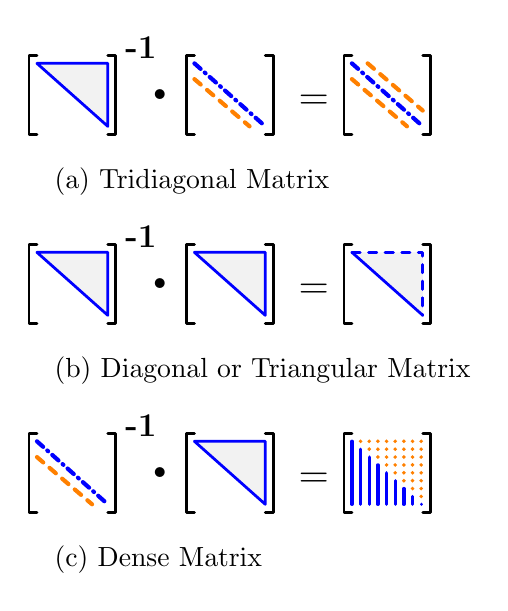
\begin{tikzpicture}[scale=1,line cap=round,line join=round,x=1.0cm,y=1.0cm]	
		\def\dx{2};
		\def\dy{-2.4};
		
		\foreach \i in {1, 2, 3}
		{
			\draw[line width=1.0] (0.1+\i*\dx,0+\dy) -- (0+\i*\dx,0+\dy) -- (0+\i*\dx,1+\dy) -- (0.1+\i*\dx,1+\dy);
			\draw[line width=1.0] (1.0+\i*\dx,0+\dy) -- (1.1+\i*\dx,0+\dy) -- (1.1+\i*\dx,1+\dy) -- (1.0+\i*\dx,1+\dy);
		}

		
		\draw[line width=1, color=blue, fill=gray!10] (0.1+\dx, 0.9+\dy) -- (1.0+\dx, 0.9+\dy) -- (1.0+\dx, 0.1+\dy) -- cycle;
		
		\draw[dash dot,line width=1.5, color=blue] (0.1+2*\dx,0.9+\dy) -- (1.+2*\dx,0.1+\dy);
		\draw[dashed,line width=1.5, color=orange] (0.1+2*\dx,0.7+\dy) -- (0.8+2*\dx,0.1+\dy);
		
		\draw[dash dot,line width=1.5, color=blue] (0.1+3*\dx,0.9+\dy) -- (1.+3*\dx,0.1+\dy);
		\draw[dashed,line width=1.5, color=orange] (0.1+3*\dx,0.7+\dy) -- (0.8+3*\dx,0.1+\dy);
		\draw[dashed,line width=1.5, color=orange] (0.3+3*\dx,0.9+\dy) -- (1.0+3*\dx,0.3+\dy);

		\node[right] at (1.1+\dx, 1.1+\dy) {\large \textbf{-1}};		
		\node[right] at (1.4+\dx, 0.5+\dy) {\Huge \textbf{.} };		
		\node[right] at (1.3+2*\dx, 0.4+\dy) {\Large = };

		\node[right] at (0.2+\dx, -0.6+\dy) {(a) Tridiagonal Matrix};		

		%%%% 2. Multiplication
		\foreach \i in {1, 2, 3}
		{
			\draw[line width=1.0] (0.1+\i*\dx,0+2*\dy) -- (0+\i*\dx,0+2*\dy) -- (0+\i*\dx,1+2*\dy) -- (0.1+\i*\dx,1+2*\dy);
			\draw[line width=1.0] (1.0+\i*\dx,0+2*\dy) -- (1.1+\i*\dx,0+2*\dy) -- (1.1+\i*\dx,1+2*\dy) -- (1.0+\i*\dx,1+2*\dy);
		}
		\draw[line width=1, color=blue, fill=gray!10] (0.1+\dx, 0.9+2*\dy) -- (1.0+\dx, 0.9+2*\dy) -- (1.0+\dx, 0.1+2*\dy) -- cycle;

		\draw[line width=1, color=blue, fill=gray!10] (0.1+2*\dx, 0.9+2*\dy) -- (1.0+2*\dx, 0.9+2*\dy) -- (1.0+2*\dx, 0.1+2*\dy) -- cycle;

		\fill[fill=gray!10] (0.1+3*\dx, 0.9+2*\dy) -- (1.0+3*\dx, 0.9+2*\dy) -- (1.0+3*\dx, 0.1+2*\dy) -- cycle;
		\draw[dashed, line width=1, color=blue] (0.1+3*\dx, 0.9+2*\dy) -- (1.0+3*\dx, 0.9+2*\dy) -- (1.0+3*\dx, 0.1+2*\dy);
		\draw[solid, line width=1, color=blue] (0.1+3*\dx, 0.9+2*\dy) -- (1.0+3*\dx, 0.1+2*\dy);
		
		\node[right] at (1.1+\dx, 1.1+2*\dy) {\large \textbf{-1}};		
		\node[right] at (1.4+\dx, 0.5+2*\dy) {\Huge \textbf{.} };		
		\node[right] at (1.3+2*\dx, 0.4+2*\dy) {\Large = };

		\node[right] at (0.2+\dx, -0.6+2*\dy) {(b) Diagonal or Triangular Matrix};		


		%%%% 3. Multiplication
		\foreach \i in {1, 2, 3}
		{
		\draw[line width=1.0] (0.1+\i*\dx,0+3*\dy) -- (0+\i*\dx,0+3*\dy) -- (0+\i*\dx,1+3*\dy) -- (0.1+\i*\dx,1+3*\dy);
		\draw[line width=1.0] (1.0+\i*\dx,0+3*\dy) -- (1.1+\i*\dx,0+3*\dy) -- (1.1+\i*\dx,1+3*\dy) -- (1.0+\i*\dx,1+3*\dy);
		}
		

		\draw[dash dot,line width=1.5, color=blue] (0.1+\dx,0.9+3*\dy) -- (1.0+\dx,0.1+3*\dy);
		\draw[dashed,line width=1.5, color=orange] (0.1+\dx,0.7+3*\dy) -- (0.8+\dx,0.1+3*\dy);
		
		\draw[line width=1, color=blue, fill=gray!10] (0.1+2*\dx, 0.9+3*\dy) -- (1.0+2*\dx, 0.9+3*\dy) -- (1.0+2*\dx, 0.1+3*\dy) -- cycle;

			
		\draw[line width=1.2, color=blue] (0.1+3*\dx, 0.9+3*\dy) -- (0.1+3*\dx, 0.1+3*\dy);
		\foreach \i in {1, ..., 8}
		{
			\draw[line width=1.2, color=blue] (0.1+\i*0.11+3*\dx, 0.9-\i*0.1+3*\dy) -- (0.1+\i*0.11+3*\dx, 0.1+3*\dy);
			\foreach \j in {1, ..., \i}
			{
				\fill [line width=1.0, color=orange] (0.1+\i*0.11 +3*\dx, 1.0 -0.1*\j +3*\dy) circle [radius = 0.025];	
			}
		}
		

		
		\node[right] at (1.1+\dx, 1.1+3*\dy) {\large \textbf{-1}};		
		\node[right] at (1.4+\dx, 0.5+3*\dy) {\Huge \textbf{.} };		
		\node[right] at (1.3+2*\dx, 0.4+3*\dy) {\Large = };
		
		\node[right] at (0.2+\dx, -0.6+3*\dy) {(c) Dense Matrix};	

		
	\end{tikzpicture}
	\caption{Matrix shapes of alternative RLC circuit ladders.}
	\label{fig:matrix_multiplication}
\end{figure}

\begin{figure*}[t!]
	\centering
	\subfloat[Input Signals]{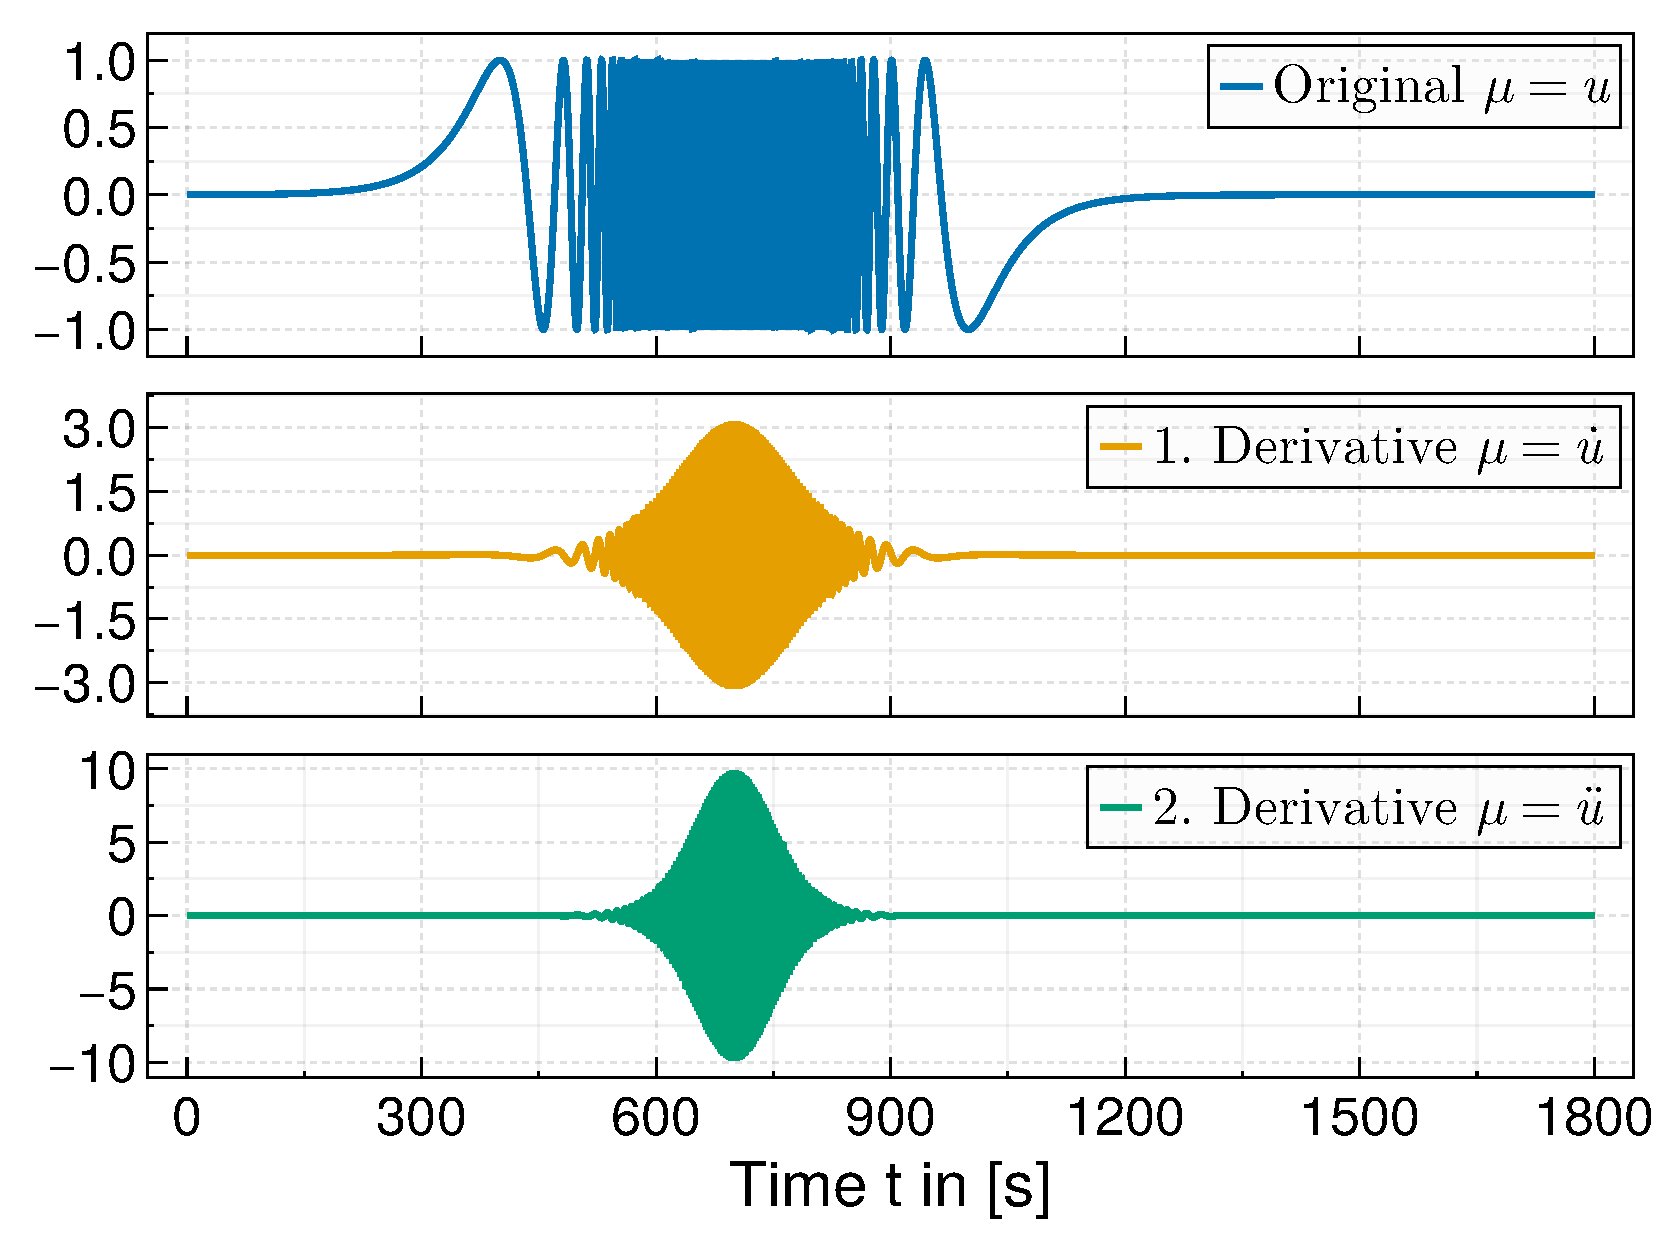
\includegraphics[width=0.99\columnwidth]{images/input_signal}}\quad
	\subfloat[Capacitor]{
\includegraphics[width=0.99\columnwidth]{images/lines_shunt_capacitor}}
	
	\subfloat[Resistor]{
\includegraphics[width=0.99\columnwidth]{images/lines_shunt_resistor}}\quad
	\subfloat[Inductor]{
\includegraphics[width=0.99\columnwidth]{images/lines_shunt_inductor}}
	\caption{Input signals and resulting states for Capacitor, Resistor and Inductor.}
	\label{fig:input_output_results}
\end{figure*}


% Idee: Tabelle mit M, D, S für unterschiedliche Schaltungen



%\begin{thebibliography}{99}
%\end{thebibliography}
	 
	%%%%%%%%%%%%%%%%%%%%%%%%%%%%%%%%%%%%%%%%%%%%%%%%%%%%%%%%%%%%%%%%%%%%%%%%%%%%%%%%%%%%%%%%%%%%%%%%%%

\section*{Acknowledgments}	
This article is inspired by student projects and theses at the University of Applied Sciences Ravensburg-Weingarten, which were supervised by Lothar Berger and the S. Scholz.

\begin{table*}[t]
	\renewcommand{\arraystretch}{1.3}
	\centering
	\caption{\MakeUppercase{General Overview}}
	\begin{tabular}{l | l c c c}
		\toprule
		 & Description & Capacitor  & Resistor & Inductor\\
		\midrule
		\textbf{Operators} & & & & \\
		$\mathcal{F}_{m}\{i_{m,n}\}$ & Main Branch & $R_{n} + L_{n} ~ \partial_t $ & $ L_n ~ \partial_{t}  + \frac{1}{C_{n}} ~ \int_{0}^{t} \cdot d\tau$ & $R_n  + \frac{1}{C_{n}} ~ \int_{0}^{t} \cdot d\tau$ \\
		$\mathcal{F}_{s}\{i_{s,n}\}$ & Shunt & $\frac{1}{C_{n}} ~ \int_{0}^{t} \cdot d\tau$ & $R_{n}$ & $L_{n} ~ \partial_t$ \\
		 & & & & \\
		\textbf{Matrix Entries} & & & & \\
		\bottomrule
	\end{tabular}
	\label{table:general_overview}
\end{table*}




%\begin{figure}[t!]
%	\begin{tikzpicture}[scale=1,line cap=round,line join=round,x=1.0cm,y=1.0cm]	
	%		
	%		\fill[color=green!20,opacity=10, rounded corners] (0.1,-1.7) rectangle (4.9,0.3);
	%		
	%		\draw[line width=1.3, color=gray] (0,0) -- (0.5,0);
	%		\draw[line width=1.3, color=gray] (1.5,0) -- (2.0,0);
	%		\draw[line width=1.3, color=gray] (2.9,0) -- (5.0,0);
	%		\draw[line width=1.3, color=gray] (4.3,0) -- (4.3,-0.7);
	%		\draw[line width=1.3, color=gray] (4.3,-0.9) -- (4.3,-1.5);
	%		\draw[line width=1.3, color=gray] (0,-1.5) -- (5.,-1.5);
	%		
	%		% Connector nodes
	%		\draw [line width=1.0] (-0.1, 0) circle [radius = 0.1];
	%		\draw [line width=1.0] ( 5.1, 0) circle [radius = 0.1];
	%		\draw [line width=1.0] (-0.1,-1.5) circle [radius = 0.1];
	%		\draw [line width=1.0] ( 5.1,-1.5) circle [radius = 0.1];
	%		
	%		% Resistor
	%		\draw[line width=2, color=blue,rounded corners] (0.5,-0.25) rectangle (1.5,0.25);
	%		
	%		% Inductor
	%		\draw[line width=2, color=blue] (2.0,0.) arc ( 180:0:0.15);
	%		\draw[line width=2, color=blue] (2.3,0.) arc ( 180:0:0.15);
	%		\draw[line width=2, color=blue] (2.6,0.) arc ( 180:0:0.15);
	%		
	%		% Capacitor
	%		\draw[line width=2, color=blue]  (4.0,-0.7) -- (4.6,-0.7);
	%		\draw[line width=2, color=blue]  (4.0,-0.9) -- (4.6,-0.9);
	%		
	%		\node at ( 1., -0.55) {$R_{1}$};
	%		\node at ( 2.45, -0.4) {$L_{1}$};
	%		\node at ( 3.7, -0.8) {$C_{1}$};
	%		
	%		
	%		% Currents
	%		\draw [->, line width=1.3, color=magenta] (3.1,0.05) -- (3.9,0.05);
	%		\draw [->, line width=1.3, color=magenta] (4.4,0.05) -- (4.9,0.05);
	%		\draw [->, line width=1.3, color=magenta] (4.25,-0.1) -- (4.25,-0.6);
	%		\node at (3.5, 0.25) {$i_{m,1}$};
	%		\node at (4.7, 0.25) {$i_{m,2}$};
	%		\node at (4.0, -0.3) {$i_{s,1}$};
	%		
	%		% Voltages
	%		\draw [->, line width=1.3, color=olive]	(-0.1, -0.2) -- (-0.1, -1.3);
	%		\draw [->, line width=1.3, color=olive]	( 5.1, -0.2) -- ( 5.1, -1.3);
	%		\draw [->, line width=1.3, color=olive]	( 0.45, 0.5) -- ( 2.95, 0.5);
	%		\node at (-0.3, -0.7) {$u$};
	%		\node at ( 5.4, -0.7)  {$z_{1}$};
	%		\node at ( 1.6, 0.7) {$v_{1}$};
	%		
	%		\node[right] at (1.0, -2.2) {(a) Single RLC Circuit with Capacitor as Shunt};
	%		
	%		\def\doff{3};
	%		\draw[line width=1.3, color=gray] (0  , 0-\doff) -- (0.3, 0-\doff);
	%		\draw[line width=1.3, color=gray] (0  ,-1-\doff) -- (0.3,-1-\doff);
	%		\draw[line width=1.3, color=gray] (1.2, 0-\doff) -- (1.6, 0-\doff);
	%		\draw[line width=1.3, color=gray] (1.2,-1-\doff) -- (1.6,-1-\doff);
	%		\draw[line width=1.3, color=gray] (1.8, 0-\doff) -- (2.3, 0-\doff);
	%		\draw[line width=1.3, color=gray] (1.8,-1-\doff) -- (2.3,-1-\doff);
	%		\draw[line width=1.3, color=gray] (3.2, 0-\doff) -- (3.6, 0-\doff);
	%		\draw[line width=1.3, color=gray] (3.2,-1-\doff) -- (3.6,-1-\doff);			
	%		\draw[line width=1.3, color=gray] (3.8, 0-\doff) -- (4.1, 0-\doff);
	%		\draw[line width=1.3, color=gray] (3.8,-1-\doff) -- (4.1,-1-\doff);			
	%		\draw[line width=1.3, color=gray] (4.3, 0-\doff) -- (4.6, 0-\doff);
	%		\draw[line width=1.3, color=gray] (4.3,-1-\doff) -- (4.6,-1-\doff);
	%		\draw[line width=1.3, color=gray] (4.8, 0-\doff) -- (5.5, 0-\doff);
	%		\draw[line width=1.3, color=gray] (4.8,-1-\doff) -- (5.5,-1-\doff);
	%		\draw[line width=1.3, color=gray] (6.4, 0-\doff) -- (6.7, 0-\doff);
	%		\draw[line width=1.3, color=gray] (6.4,-1-\doff) -- (6.7,-1-\doff);	
	%		
	%		\draw [line width=1.0] (-0.1, 0-\doff) circle [radius = 0.1];
	%		\draw [line width=1.0] (-0.1,-1-\doff) circle [radius = 0.1];
	%		
	%		\draw [line width=1.0] ( 1.7, 0-\doff) circle [radius = 0.1];
	%		\draw [line width=1.0] ( 1.7,-1-\doff) circle [radius = 0.1];
	%		
	%		\draw [line width=1.0] ( 3.7, 0-\doff) circle [radius = 0.1];
	%		\draw [line width=1.0] ( 3.7,-1-\doff) circle [radius = 0.1];
	%		
	%		\draw [line width=1.0] ( 4.7, 0-\doff) circle [radius = 0.1];
	%		\draw [line width=1.0] ( 4.7,-1-\doff) circle [radius = 0.1];
	%		
	%		\draw [line width=1.0] ( 6.8, 0-\doff) circle [radius = 0.1];
	%		\draw [line width=1.0] ( 6.8,-1-\doff) circle [radius = 0.1];
	%		
	%		\draw [line width=1.0] (4,   -0.2-\doff) -- (4.25, 0.2-\doff);	
	%		\draw [line width=1.0] (4.15,-0.2-\doff) -- (4.4 , 0.2-\doff);	
	%		\draw [line width=1.0] (4,   -1.2-\doff) -- (4.25,-0.8-\doff);	
	%		\draw [line width=1.0] (4.15,-1.2-\doff) -- (4.4 ,-0.8-\doff);		
	%		
	%		\draw[dashed,line width=2,rounded corners, fill=green!20] (0.3,-1.3-\doff) rectangle (1.2,0.3-\doff);
	%		\draw[dashed,line width=2,rounded corners, fill=green!20] (2.3,-1.3-\doff) rectangle (3.2,0.3-\doff);
	%		\draw[dashed,line width=2,rounded corners, fill=green!20] (5.5,-1.3-\doff) rectangle (6.4,0.3-\doff);
	%		
	%		\node at (0.77,-0.2-\doff) {RLC};
	%		\node at (0.77,-0.6-\doff) {\textbf{1}};
	%		
	%		\node at (2.77,-0.2-\doff) {RLC};
	%		\node at (2.77,-0.6-\doff) {\textbf{2}};
	%		
	%		\node at (5.97,-0.2-\doff) {RLC};
	%		\node at (5.97,-0.6-\doff) {\textbf{N}};
	%		
	%		% Voltages
	%		\draw [->, line width=1.3, color=olive]	(-0.1, -0.2-\doff) -- (-0.1, -0.8-\doff);
	%		\draw [->, line width=1.3, color=olive]	( 1.7, -0.2-\doff) -- ( 1.7, -0.8-\doff);
	%		\draw [->, line width=1.3, color=olive]	( 3.7, -0.2-\doff) -- ( 3.7, -0.8-\doff);
	%		\draw [->, line width=1.3, color=olive]	( 4.7, -0.2-\doff) -- ( 4.7, -0.8-\doff);
	%		\draw [->, line width=1.3, color=olive]	( 6.8, -0.2-\doff) -- ( 6.8, -0.8-\doff);
	%		\node at (-0.3, -0.5-\doff) {$u$};
	%		\node at ( 1.9, -0.5-\doff) {$z_{1}$};
	%		\node at ( 3.9, -0.5-\doff) {$z_{2}$};
	%		\node at ( 5.1, -0.5-\doff) {$z_{N-1}$};
	%		\node at ( 7.0, -0.5-\doff)  {$y$};
	%		
	%		\node[right] at (1.0, -2-\doff) {(b) Composition of single circuits};
	%		
	%	\end{tikzpicture}
%	\caption{Ladder of RLC Circuits. The voltage at the last shunt is the output, $z_{n} = y$.}
%	\label{fig:cascaded_rlc}
%	
%\end{figure}

%\begin{figure}[t!]
%	\centering
%	\begin{tikzpicture}[scale=1,line cap=round,line join=round,x=1.0cm,y=1.0cm]	
	%		%%% 1. Circuit: Resistor as Shunt %%%%%
	%		%%% 1. Circuit: Resistor as Shunt %%%%%
	%		%%% 1. Circuit: Resistor as Shunt %%%%%
	%		\draw[line width=1.3, color=gray] (0,0) -- (0.5,0);
	%		\draw[line width=1.3, color=gray] (1.4,0) -- (2.0,0);
	%		\draw[line width=1.3, color=gray] (2.2,0) -- (4.0,0);
	%		\draw[line width=1.3, color=gray] (3.1,0) -- (3.1,-0.3);
	%		\draw[line width=1.3, color=gray] (3.1,-1.3) -- (3.1,-1.6);
	%		\draw[line width=1.3, color=gray] (0,-1.6) -- (4.0,-1.6);
	%		
	%		
	%		% Nodes
	%		\draw [line width=1.0] (-0.1, 0) circle [radius = 0.1];
	%		\draw [line width=1.0] ( 4.1, 0) circle [radius = 0.1];
	%		\draw [line width=1.0] (-0.1,-1.6) circle [radius = 0.1];
	%		\draw [line width=1.0] ( 4.1,-1.6) circle [radius = 0.1];
	%		
	%		% Voltages
	%		\draw [->, line width=1.3, color=olive]	(-0.1, -0.2) -- (-0.1, -1.4);
	%		\draw [->, line width=1.3, color=olive]	( 4.1, -0.2) -- ( 4.1, -1.4);
	%		\draw [->, line width=1.3, color=olive]	( 0.45, 0.5) -- ( 2.3, 0.5);
	%		\node at (-0.3, -0.7) {$z_{n}$};
	%		\node at ( 4.6, -0.7)  {$z_{n+1}$};
	%		\node at ( 1.6, 0.7) {$v_{n}$};
	%		
	%		% Inductor
	%		\draw[line width=2, color=blue] (0.5,0.) arc ( 180:0:0.15);
	%		\draw[line width=2, color=blue] (0.8,0.) arc ( 180:0:0.15);
	%		\draw[line width=2, color=blue] (1.1,0.) arc ( 180:0:0.15);
	%		
	%		% Capacitor
	%		\draw[line width=2, color=blue] (2.0,-0.2) -- (2.0,0.2);
	%		\draw[line width=2, color=blue] (2.2,-0.2) -- (2.2,0.2);
	%		
	%		% Resistor
	%		\draw[line width=2, color=blue,rounded corners] (2.9,-0.3) rectangle (3.3,-1.3);
	%		
	%		\node at ( 1., -0.5) {$L_{n}$};
	%		\node at ( 2.1, -0.5) {$C_{n}$};
	%		\node at ( 2.6, -0.9) {$R_{n}$};
	%		
	%		\node[right] at (0.5, -2) {(a) Resistor as Shunt};
	%		
	%		%%% 2. Circuit: Inductor as Shunt %%%%%
	%		%%% 2. Circuit: Inductor as Shunt %%%%%
	%		%%% 2. Circuit: Inductor as Shunt %%%%%
	%		
	%		\def\doff{-3.5};
	%		
	%		\draw[line width=1.3, color=gray] (0,0+\doff) -- (0.5,0+\doff);
	%		\draw[line width=1.3, color=gray] (1.4,0+\doff) -- (2.0,0+\doff);
	%		\draw[line width=1.3, color=gray] (2.2,0+\doff) -- (4.0,0+\doff);
	%		\draw[line width=1.3, color=gray] (3.1,0+\doff) -- (3.1,-0.3+\doff);
	%		\draw[line width=1.3, color=gray] (3.1,-1.2+\doff) -- (3.1,-1.6+\doff);
	%		\draw[line width=1.3, color=gray] (0,-1.6+\doff) -- (4.0,-1.6+\doff);
	%		
	%		% Nodes
	%		\draw [line width=1.0] (-0.1, 0+\doff) circle [radius = 0.1];
	%		\draw [line width=1.0] ( 4.1, 0+\doff) circle [radius = 0.1];
	%		\draw [line width=1.0] (-0.1,-1.6+\doff) circle [radius = 0.1];
	%		\draw [line width=1.0] ( 4.1,-1.6+\doff) circle [radius = 0.1];
	%		
	%		% Voltages
	%		\draw [->, line width=1.3, color=olive]	(-0.1, -0.2+\doff) -- (-0.1, -1.4+\doff);
	%		\draw [->, line width=1.3, color=olive]	( 4.1, -0.2+\doff) -- ( 4.1, -1.4+\doff);
	%		\draw [->, line width=1.3, color=olive]	( 0.45, 0.5+\doff) -- ( 2.3, 0.5+\doff);
	%		\node at (-0.3, -0.7+\doff) {$z_{n}$};
	%		\node at ( 4.6, -0.7+\doff)  {$z_{n+1}$};
	%		\node at ( 1.6, 0.7+\doff) {$v_{n}$};
	%		
	%		% Resistor
	%		\draw[line width=2, color=blue,rounded corners] (0.5,-0.2+\doff) rectangle (1.4,0.2+\doff);
	%		
	%		% Capacitor
	%		\draw[line width=2, color=blue] (2.0,-0.2+\doff) -- (2.0,0.2+\doff);
	%		\draw[line width=2, color=blue] (2.2,-0.2+\doff) -- (2.2,0.2+\doff);
	%		
	%		% Inductor
	%		\draw[line width=2, color=blue] (3.1,-0.3+\doff) arc ( 90:-90:0.15);
	%		\draw[line width=2, color=blue] (3.1,-0.6+\doff) arc ( 90:-90:0.15);
	%		\draw[line width=2, color=blue] (3.1,-0.9+\doff) arc ( 90:-90:0.15);
	%		
	%		
	%		\node at ( 1., -0.5+\doff) {$R_{n}$};
	%		\node at ( 2.1, -0.5+\doff) {$C_{n}$};
	%		\node at ( 2.8, -0.9+\doff) {$L_{n}$};
	%		
	%		\node[right] at (0.5, -2+\doff) {(b) Inductor as Shunt};	
	%	\end{tikzpicture}
%	\caption{Single RLC circuits with Resistor (a) or Inductor (b) as Shunt.}
%	\label{fig:rlc_resistor_inductor}
%\end{figure}


%
%and consequently, we derive the relationship
%\begin{align}
%	z_{n-1}(t) =&~ v_{n}(t) + z_{n}(t) = \mathcal{F}_{m,n} \left\{i_{m,n}\right\}(t) + z_{n}(t) \nonumber \\
%	=&~ \mathcal{F}_{m,n} \left\{i_{m,n+1} + i_{s,n}\right\}(t) + z_{n}(t) \nonumber \\
%	=&~ \mathcal{F}_{m,n} \left\{i_{m,n+1} +  \mathcal{F}^{-1}_{s,n} \left\{z_{n}\right\} \right\}(t) + z_{n}(t) \nonumber \\
%	=&~ L_{n} C_{n} ~ \partial_{t}^2 z_{n}(t) + R_{n} C_{n} ~ \partial_{t} z_{n}(t) + z_{n}(t) \nonumber \\
%	&\qquad \qquad \qquad+ \mathcal{F}_{m,n} \left\{i_{m,n+1} \right\}(t) \text{.} \label{eq:shunt_vol_rel_circuit_n}
%\end{align}
%Here, we face the issue that we need to evaluate the equations of a subsequent circuit $n+1$ to yield $\mathcal{F}_{m,n} \left\{i_{m,n+1} \right\}(t)$ in Eq. \eqref{eq:shunt_vol_rel_circuit_n}. Hence, we need to start this ... with the last circuit and go towards the first one.
%
%In the last circuit, we have a common current in the whole circuit $i_{m,N}(t) = i_{s,N}(t) = C_{N} \partial_{t} z_{N}(t)$ and so we note sum of voltages as
%\begin{align}
%	0 =&~  L_{N} C_{N} ~ \partial_{t}^2 z_{N}(t) + R_{N} C_{N} ~ \partial_{t} z_{N}(t) \nonumber \\
%	&\qquad -z_{N-1}(t) + z_{N}(t) \text{.}
%\end{align}
%Continuing with the second last circuit $N-1$, we find the voltage across $R_{N-1}$ and $L_{N-1}$ with Eq. (\ref{eq:kirchhoff_current}, \ref{eq:rlc_cap_volt_r_l}) as
%\begin{equation*}
%	v_{N-1}(t) = R_{N-1}  C_{N} ~ \partial_{t} z_{N}(t) + L_{N-1}  C_{N} ~ \partial_{t}^2 z_{N}(t)
%\end{equation*}
%% missing term as
%%\begin{align*}
%%	&\mathcal{F}_{m,N-1} \left\{i_{m,N} \right\}(t) =~ R_{N-1} ~ i_{m,N}(t) + L_{N-1} ~ \partial_{t} i_{m,N}(t) \\
%%	&\quad=~ R_{N-1}  C_{N} ~ \partial_{t} z_{N}(t) + L_{N-1}  C_{N} ~ \partial_{t}^2 z_{N}(t)	
%%\end{align*}
%and in accordance with Eq. \eqref{eq:shunt_vol_rel_circuit_n}, we yield the sum of voltages
%\begin{align*}
%	0 =&~ L_{N-1} C_{N} ~ \partial_{t}^2 z_{N}(t) + L_{N-1} C_{N-1} ~ \partial_{t}^2 z_{N-1}(t)  \\
%		&~ + R_{N-1} C_{N} ~ \partial_{t} z_{N}(t)  + R_{N-1} C_{N-1} ~ \partial_{t} z_{N-1}(t)  \\ 
%		&~ -z_{N-2}(t) + z_{N-1}(t) \text{.} 
%\end{align*}
%We continue this procedure and we calculate for the $n$-th circuit, $n\in\{2,\ldots,N\}$ the differential equation
%\begin{equation*}
%	0 =~ \sum_{k=n}^{N} \left[ L_{n} C_{k} ~ \partial_{t}^2 z_{k}(t) + R_{n} C_{k} ~ \partial_{t} z_{k}(t)  \right] + z_{n}(t) - z_{n-1}(t) \text{.} 
%\end{equation*}
%For the first circuit, we have $u(t) = z_{0}(t)$ and so we note
%\begin{equation*}
%	u(t) =~ \sum_{k=1}^{N} \left[ L_{1} C_{k} ~ \partial_{t}^2 z_{k}(t) + R_{1} C_{k} ~ \partial_{t} z_{k}(t)  \right] + z_{1}(t) \text{.} 
%\end{equation*}


%\begin{table}[b]
%	\renewcommand{\arraystretch}{1.3}
%	\centering
%	\caption{\MakeUppercase{Overview Voltage Operators}}
%	\begin{tabular}{l | c c}
%		\toprule
%		Shunt & Main Branch $\mathcal{F}_{m}\{i_{m}\}$ & Shunt   $\mathcal{F}_{s,n}\{i_{s}\}$ \\
%		\midrule
%		Capacitor & $R_{n} + L_{n} \partial_t $ & $\frac{1}{C_{n}} \int_{0}^{t} \cdot d\tau$ \\
%		Resistor & & \\
%		Inductor & &
%		\\
%		\bottomrule
%	\end{tabular}
%	\label{table:overview_voltage_operators}
%\end{table}


\end{document}
